% Chapter 12 — Dynamic Scheduling, CUDA Graphs, and Device-Initiated Kernel Orchestration
% Style follows chapter01/02 presentations (LaTeX Beamer, Madrid, navy).
% Compile: pdflatex chapter12-presentation.tex  (run twice)
\documentclass[aspectratio=169]{beamer}

% ====== Presenter info: EDIT ME ======
\newcommand{\PresenterName}{Your Name}          % <-- 改成你的名字
\newcommand{\PresenterTitle}{Applied Scientist} % <-- 改成你的头衔
\newcommand{\PresenterOrg}{AWS}
% =====================================

\usetheme{Madrid}
\definecolor{navy}{RGB}{18,47,90}
\definecolor{kwblue}{RGB}{0,56,132}
\definecolor{okgreen}{RGB}{80,130,20}
\usecolortheme[named=navy]{structure}
\setbeamercolor{frametitle}{bg=navy,fg=white}
\setbeamercolor{title}{bg=navy,fg=white}
\setbeamercolor{block title}{bg=navy,fg=white}
\setbeamercolor{block body}{bg=gray!12,fg=black}
\setbeamercolor{block title example}{bg=okgreen,fg=white}
\setbeamercolor{block body example}{bg=okgreen!10,fg=black}
\setbeamertemplate{navigation symbols}{}
\setbeamertemplate{blocks}[rounded][shadow=true]

\usepackage{booktabs}
\usepackage{listings}
\lstset{
  language=C++,
  basicstyle=\ttfamily\fontsize{6.5}{7.6}\selectfont,
  keywordstyle=\color{kwblue}\bfseries,
  commentstyle=\color{gray}\itshape,
  stringstyle=\color{okgreen},
  showstringspaces=false,
  breaklines=true,
  columns=fullflexible
}

\newcommand{\kw}[1]{\textbf{\textcolor{kwblue}{#1}}}
\newcommand{\pe}[1]{{\footnotesize\itshape Plain English: #1}}
\newcommand{\refmark}[1]{\textsuperscript{[#1]}}

\title[AI Systems Performance Engineering]{AI Systems Performance Engineering}
\subtitle{Chapter 12 --- Dynamic Scheduling, CUDA Graphs, and Device-Initiated Kernel Orchestration}
\author[\PresenterName\ \ \PresenterTitle\ \ \PresenterOrg]{\PresenterName\\\PresenterTitle\\\PresenterOrg}
\institute[]{\footnotesize Internal Training for Applied Scientists on AI Infrastructure}
\date{August 15, 2026}

\begin{document}

% ---------------------------------------------------------------- 1
\begin{frame}
  \titlepage
\end{frame}

% ---------------------------------------------------------------- 2
\begin{frame}{What This Talk Is About --- and Why}
  \begin{block}{In plain English}
    Chapters 6--11 made \emph{individual kernels} fast. But between kernels, the GPU often sits idle,
    \kw{waiting for the CPU} to decide what to run next. This chapter moves the \kw{scheduling itself onto
    the GPU}: work queues built from atomics, whole pipelines replayed as \kw{CUDA Graphs}, kernels that
    launch other kernels --- and, across many GPUs, \kw{NVSHMEM} so devices talk without the CPU at all.
  \end{block}
  \begin{columns}[t]
    \column{0.48\textwidth}
    \begin{itemize}
      \item \kw{The problem:} launch overhead and CPU round trips leave idle gaps between kernels ---
            microseconds that add up to real money at LLM scale.
      \item \kw{The goal:} keep every SM fed, end to end, with the host \kw{off the critical path}.
    \end{itemize}
    \column{0.48\textwidth}
    \begin{itemize}
      \item \kw{The tools:} atomic work queues, CUDA Graphs (host- and device-launched),
            conditional nodes, dynamic parallelism, NCCL + NVSHMEM.
      \item \kw{The compass:} roofline analysis tells us which tool moves the needle.
    \end{itemize}
  \end{columns}
  \medskip
  \centering\footnotesize\itshape
  This is what vLLM, TensorRT-LLM, and PyTorch do under the hood --- worth understanding first-hand.
\end{frame}

% ---------------------------------------------------------------- 3
\begin{frame}{Roadmap}
  \begin{enumerate}
    \item \kw{Dynamic scheduling} --- atomic counters and work queues that balance uneven work
    \item \kw{CUDA Graphs} --- capture once, replay forever; dynamic updates
    \item \kw{Device-initiated graphs} --- fire-and-forget / tail / sibling launches; conditional nodes
    \item \kw{Dynamic parallelism} --- kernels spawning kernels for data-dependent work
    \item \kw{Multi-GPU orchestration} --- peer copies, NCCL in graphs, NVSHMEM one-sided ops
    \item \kw{Roofline-guided decisions} --- which technique for which bottleneck
  \end{enumerate}
  \medskip
  \pe{one theme, six tools: get the CPU out of the loop so the GPU never waits.}
\end{frame}

% ---------------------------------------------------------------- 4
\begin{frame}{The Enemy: Uneven Work $\Rightarrow$ Idle SMs}
  \begin{columns}[c]
    \column{0.55\textwidth}
    \begin{itemize}
      \item Input-dependent loops give threads \kw{different amounts of work}:
            fast blocks finish, their SMs \kw{idle} while stragglers grind on.
      \item By the time the longest block finishes, much of the GPU has done nothing for a while ---
            \kw{low achieved occupancy}, wasted cycles.
      \item Diagnose it: \kw{Nsight Systems} shows the timeline gaps;
            \kw{Nsight Compute}'s \emph{SM Active} \% shows cycles with zero active warps;
            add \kw{NVTX} ranges to tie gaps to code.
    \end{itemize}
    \column{0.42\textwidth}
    \begin{block}{The takeaway}
      Static, preassigned work only balances \emph{uniform} workloads.
      For irregular work, assignment must happen \kw{at runtime, on the device}.
    \end{block}
  \end{columns}
  \medskip
  \pe{if you deal every worker a fixed stack of tasks, the lucky ones go home early while the unlucky ones work overtime --- and you pay for the whole factory either way.}
\end{frame}

% ---------------------------------------------------------------- 5
\begin{frame}[fragile]{Atomic Counters: Fast, but Watch the Contention}
  \begin{columns}[c]
    \column{0.52\textwidth}
    \begin{itemize}
      \item Global atomics are serviced \kw{in the L2 cache} --- fast when uncontended, but
            under contention threads \kw{serialize} at one address.
      \item Metric: \kw{\texttt{atomic\_transactions\_per\_request}} (Nsight Compute):
            $\approx 1.0$ ideal; $> 1.0$ = stall-and-retry.
      \item Fix: \kw{amortize} --- one atomic per \kw{batch}, not per item:
    \end{itemize}
\begin{lstlisting}
// Before: one atomic per item
int idx = atomicAdd(&queue_head, 1);
if (idx < N) process(data[idx]);
// After: one atomic per 32 items
int start = atomicAdd(&queue_head, 32);
for (int i = start; i < start + 32 && i < N; ++i)
    process(data[i]);
\end{lstlisting}
    \column{0.44\textwidth}
    \centering
    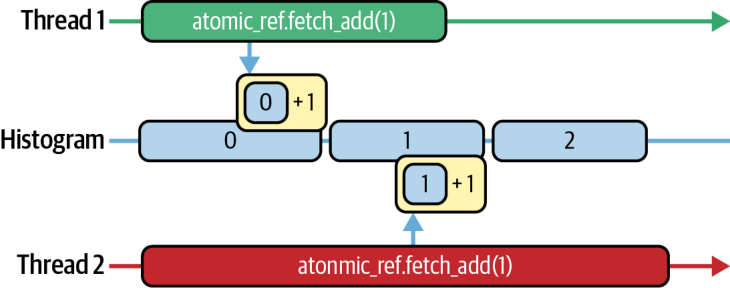
\includegraphics[width=\linewidth]{figs/fig12-1.png}\\
    {\scriptsize Figure 12-1. On-chip (L2) atomic adds from multiple threads}
    \medskip
    \begin{itemize}\small
      \item Even batch size \kw{8--16} kills most contention, thanks to L2 bandwidth.
    \end{itemize}
  \end{columns}
  \smallskip
  \pe{send one runner per crew to fetch 32 tickets at once, instead of everyone queuing at the window.}
\end{frame}

% ---------------------------------------------------------------- 6
\begin{frame}[fragile]{Atomic Work Queues: Load Balancing on the Device}
  \begin{columns}[c]
    \column{0.52\textwidth}
\begin{lstlisting}
__device__ unsigned int globalIndex = 0;
__global__ void computeKernelDynamicBatch(...) {
  int lane = threadIdx.x & (warpSize - 1);
  while (true) {
    unsigned mask = __activemask();
    int leader = __ffs(mask) - 1;
    unsigned base = 0;
    if (lane == leader)              // warp leader grabs
      base = atomicAdd(&globalIndex, warpSize);
    base = __shfl_sync(mask, base, leader); // broadcast
    unsigned idx = base + lane;
    if (idx >= N) break;             // dynamic termination
    /* ... process element idx ... */
  }
}
\end{lstlisting}
    \column{0.44\textwidth}
    \centering
    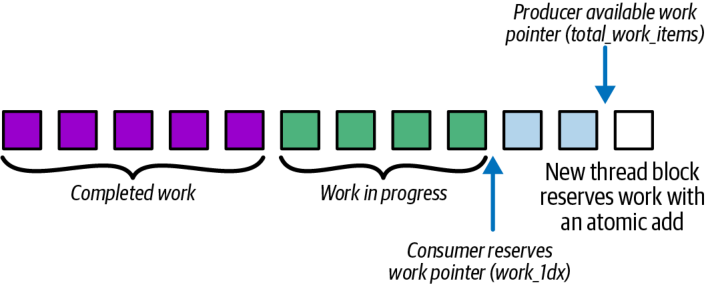
\includegraphics[width=\linewidth]{figs/fig12-2.png}\\
    {\scriptsize Figure 12-2. Atomic counter as a dynamic work queue across SMs}
    \medskip
    \begin{itemize}\small
      \item Warps that finish early \kw{immediately pull the next batch} --- no SM idles
            until the queue is drained.
    \end{itemize}
  \end{columns}
\end{frame}

% ---------------------------------------------------------------- 7
\begin{frame}{Atomic Queues: What You Gain, and When}
  \begin{columns}[c]
    \column{0.5\textwidth}
    {\small\setlength{\tabcolsep}{4pt}
    \begin{tabular}{@{}lrr@{}}
      \toprule
      & \textbf{Static} & \textbf{Dynamic} \\
      \midrule
      Runtime (skewed work) & $\sim$200 ms & \kw{$\sim$100 ms} \\
      \bottomrule
    \end{tabular}}\\[6pt]
    \begin{itemize}\small
      \item \kw{2$\times$} in extreme imbalance; typically \kw{10--20\%} for moderate imbalance.
      \item For \emph{mild} imbalance, atomic + shuffle overhead can cancel the gains --- measure.
    \end{itemize}
    \column{0.46\textwidth}
    \begin{block}{Reach for a dynamic queue when profiling shows}
      \begin{itemize}\small
        \item warp-idle stalls / low achieved occupancy,
        \item timeline gaps from uneven per-task runtimes,
        \item \texttt{atomic\_transactions\_per\_request} $\approx 1.0$ after batching
              (i.e., the queue itself isn't the new bottleneck).
      \end{itemize}
    \end{block}
  \end{columns}
  \medskip
  \pe{no high-level PyTorch API for this --- it's a custom-CUDA-kernel technique.}
\end{frame}

% ---------------------------------------------------------------- 8
\begin{frame}{CUDA Graphs: Capture Once, Replay with One Call}
  \begin{columns}[c]
    \column{0.5\textwidth}
    \begin{itemize}
      \item Launching a pipeline of kernels + copies one-by-one pays
            \kw{CPU launch overhead every iteration}.
      \item A \kw{CUDA Graph} records the workflow --- nodes (kernels, memcpys) and
            dependency edges --- and \kw{replays it with one host call}.
      \item Dependencies known upfront $\Rightarrow$ batch scheduling, no per-step
            CPU handshakes, automatic overlap of independent nodes.
      \item Under the hood of \kw{PyTorch}, \kw{vLLM}, \kw{TensorRT-LLM}
            (one precaptured graph per batch-size bucket).\refmark{2,6}
    \end{itemize}
    \column{0.47\textwidth}
    \centering
    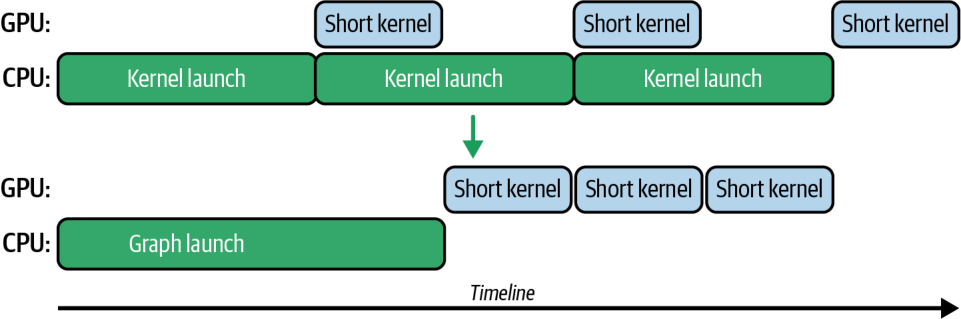
\includegraphics[width=\linewidth]{figs/fig12-3.png}\\
    {\scriptsize Figure 12-3. Launch timeline without (top) and with (bottom) CUDA Graphs}
  \end{columns}
  \medskip
  \pe{record the cooking show once and press play --- don't dictate the recipe every night.}
\end{frame}

% ---------------------------------------------------------------- 9
\begin{frame}[fragile]{Capturing a Graph: Stream Capture API}
  \begin{columns}[t]
    \column{0.55\textwidth}
\begin{lstlisting}
cudaGraph_t graph;  cudaGraphExec_t instance;
cudaStreamBeginCapture(stream, cudaStreamCaptureModeGlobal);
kernelA<<<grid, block, 0, stream>>>(d_X);
kernelB<<<grid, block, 0, stream>>>(d_Y);
kernelC<<<grid, block, 0, stream>>>(d_Z);
cudaStreamEndCapture(stream, &graph);
cudaGraphInstantiate(&instance, graph, nullptr, nullptr, 0);

for (int iter = 0; iter < 100; ++iter)
    cudaGraphLaunch(instance, stream);  // 1 call = A->B->C
cudaStreamSynchronize(stream);
\end{lstlisting}
    \column{0.42\textwidth}
    \begin{itemize}
      \item \kw{Capture}: bracket normal stream code with
            \texttt{BeginCapture}/\texttt{EndCapture} --- nothing executes during capture.
      \item \kw{Instantiate} once ($\to$ \texttt{cudaGraphExec\_t}), then \kw{launch}
            per iteration: 1 CPU call instead of 3+.
      \item Partial pipelines are fine --- capture just the repetitive subgraph.
      \item Parameters changed? \kw{\texttt{cudaGraphExecUpdate}}.
    \end{itemize}
  \end{columns}
\end{frame}

% ---------------------------------------------------------------- 10
\begin{frame}[fragile]{CUDA Graphs in PyTorch}
  \begin{columns}[t]
    \column{0.55\textwidth}
\begin{lstlisting}[language=Python]
# 1) warm-up: initialize kernels/cuBLAS lazily
_ = opC(opB(opA(X)));  torch.cuda.synchronize()
static_x.copy_(X)                  # seed static input
# 2) capture with static (pointer-stable) buffers
g = torch.cuda.CUDAGraph()
with torch.cuda.graph(g, stream=stream):
    torch.mul(static_x, 1.1, out=static_y)
    torch.add(static_y, 2.0, out=static_z)
    torch.sqrt(static_z, out=static_w)
# 3) replay: one host call per iteration
for i in range(100):
    # static_x.copy_(new_X)  # if inputs change
    g.replay()
\end{lstlisting}
    \column{0.42\textwidth}
    \begin{itemize}\small
      \item \kw{Warm-up is mandatory}: capture won't record lazy init (cuBLAS/cuDNN);
            skipping it can fail the capture.
      \item All tensors at \kw{fixed addresses, fixed shapes}: preallocate, write with
            \texttt{out=}, update inputs via \kw{\texttt{copy\_}} into static tensors.
      \item \texttt{graph\_pool\_handle()}: dedicated pool for pointer stability.
      \item No allocations, \texttt{print}, or RNG setup inside the capture.
    \end{itemize}
  \end{columns}
  \smallskip
  \pe{a graph is a videotape of GPU work --- the actors (tensors) must stand on the same marks every take.}
\end{frame}

% ---------------------------------------------------------------- 11
\begin{frame}{What Graphs Buy You --- and the Fine Print}
  \begin{columns}[c]
    \column{0.55\textwidth}
    {\small\setlength{\tabcolsep}{4pt}
    \begin{tabular}{@{}lrr@{}}
      \toprule
      \textbf{Per 100 iterations} & \textbf{Before} & \textbf{After} \\
      \midrule
      CPU launch calls & 300 & \kw{100} \\
      Host sync calls & 300 & \kw{0} \\
      GPU idle / iteration & $\sim$3 \textmu s & \kw{0} \\
      Iteration latency & 1.00 ms & \kw{0.75 ms} \\
      \bottomrule
    \end{tabular}}\\[4pt]
    {\scriptsize Table 12-1 (illustrative numbers --- see the book's GitHub repo\refmark{7})}
    \column{0.42\textwidth}
    \centering
    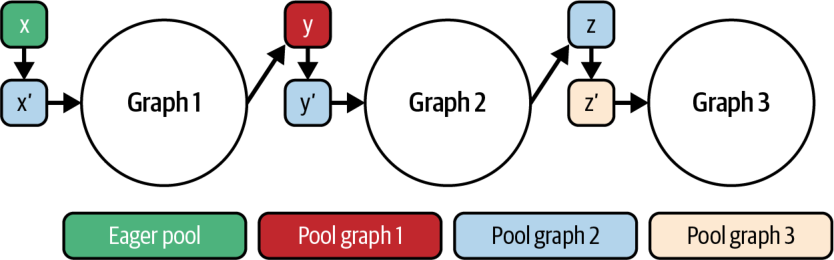
\includegraphics[width=\linewidth]{figs/fig12-4.png}\\
    {\scriptsize Figure 12-4. PyTorch backs graphs with static memory pools}
  \end{columns}
  \medskip
  \begin{itemize}
    \item Graphs don't make a single kernel faster --- they remove \kw{between-kernel} overhead.
    \item Gains grow with \kw{many small kernels} (exactly the LLM decode profile).
  \end{itemize}
\end{frame}

% ---------------------------------------------------------------- 12
\begin{frame}{Dynamic Graph Update: Don't Recapture, Patch}
  \begin{itemize}
    \item Shapes or pointers changed? \kw{\texttt{cudaGraphExecUpdate}} /
          \texttt{cudaGraphExecKernelNodeSetParams} patch grid/block dims, kernel params,
          and addresses \kw{in the existing executable graph}.
    \item Takes \kw{a few microseconds} --- preserves the sub-100 \textmu s replay path;
          incompatible edits (adding/removing nodes) return an error $\Rightarrow$ recapture.
  \end{itemize}
  \begin{block}{Typical inference workflow}
    \begin{enumerate}\small
      \item Capture a \kw{template graph} at the maximum batch size (e.g., 128).
      \item Request arrives with batch 64 $\Rightarrow$ \texttt{cudaGraphExecUpdate}
            adjusts launch dims (and buffer pointers).
      \item Replay. Structure changed (different kernel count)? Recapture once, keep updating after.
    \end{enumerate}
  \end{block}
  \medskip
  \pe{like editing the guest count on a standing catering order instead of renegotiating the contract every day.}
\end{frame}

% ---------------------------------------------------------------- 13
\begin{frame}{Device-Initiated Graph Launch: Remove the CPU Entirely}
  \begin{columns}[c]
    \column{0.55\textwidth}
    \begin{itemize}
      \item A running kernel can \kw{launch a prerecorded graph from device code}:
            \texttt{cudaGraphLaunch(graphExec, stream)} inside a kernel.
      \item Setup: instantiate with \kw{\texttt{cudaGraphInstantiateFlagDeviceLaunch}},
            then \kw{\texttt{cudaGraphUpload}} to GPU memory \emph{before} any device launch.
      \item $\sim$\kw{2$\times$ lower launch latency} than host-side graph launch ---
            and it stays \kw{flat} as the graph grows in nodes or width.\refmark{3}
      \item The GPU computes the decision \emph{and} dispatches the work --- no host round trip.
    \end{itemize}
    \column{0.42\textwidth}
    \centering
    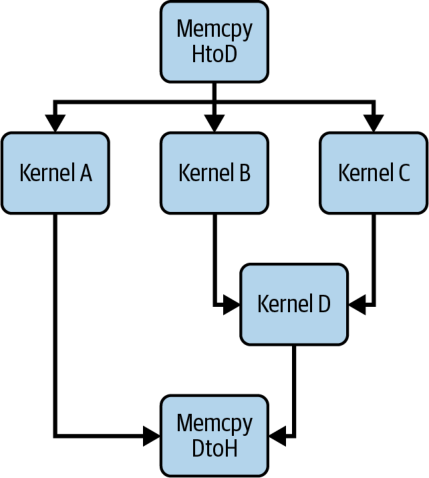
\includegraphics[width=0.72\linewidth]{figs/fig12-5.png}\\
    {\scriptsize Figure 12-5. A graph of kernels and copies with dependency edges}
  \end{columns}
  \medskip
  \pe{the factory floor schedules its own jobs --- no phoning HQ between tasks.}
\end{frame}

% ---------------------------------------------------------------- 14
\begin{frame}{Three Device-Launch Modes}
  \begin{columns}[t]
    \column{0.32\textwidth}
    \begin{block}{Fire-and-forget}
      \small Child graph starts \kw{immediately}, concurrent with the parent; parent doesn't wait.
      For independent side tasks. Limit: \kw{120} per graph execution.
    \end{block}
    \column{0.32\textwidth}
    \begin{block}{Tail launch}
      \small Runs \kw{after the parent completes} --- a continuation. Enables GPU-resident schedulers:
      a kernel can \kw{re-enqueue itself}. Limits: \kw{255} pending; one pending \kw{self}-tail-launch.
    \end{block}
    \column{0.32\textwidth}
    \begin{block}{Sibling}
      \small Fire-and-forget as a \kw{peer} of the parent graph, in the parent's stream environment ---
      runs now, without delaying the parent's tail launches.
    \end{block}
  \end{columns}
  \medskip
  \centering
  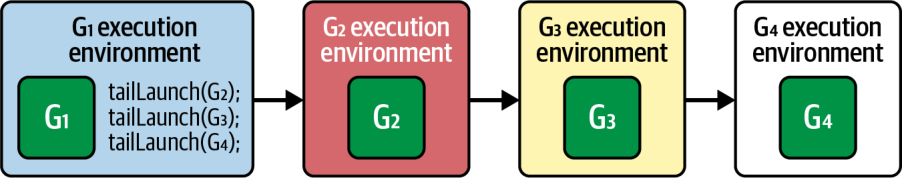
\includegraphics[width=0.6\linewidth]{figs/fig12-6.png}\\
  {\scriptsize Figure 12-6. Tail launches execute one at a time, in enqueue order}
  \medskip
  \begin{itemize}\small
    \item Need the child's results? \kw{Tail}. Independent side job? \kw{Fire-and-forget / sibling}.
  \end{itemize}
\end{frame}

% ---------------------------------------------------------------- 15
\begin{frame}{Pattern: A GPU-Resident LLM Decode Scheduler}
  \begin{block}{Atomic queue + tail launch = persistent in-kernel scheduler}
    \begin{enumerate}\small
      \item Capture the transformer block's forward pass (attention + FFN) as a \kw{decode graph}.
      \item A lightweight \kw{persistent scheduler kernel} claims work:
            \texttt{atomicAdd(\&queueHead, 1)}.
      \item It \kw{tail-launches} the precaptured decode graph for that item, then loops for the next.
    \end{enumerate}
  \end{block}
  \begin{itemize}
    \item Every token is processed start-to-finish \kw{on the device} --- the CPU never re-enters
          the critical path.
    \item Adapts on the fly: switch between precaptured graphs, or \texttt{cudaGraphExecUpdate}
          parameters for new sequence lengths / batch sizes.
    \item This is the architectural idea behind modern \kw{GPU-resident inference engines}.
  \end{itemize}
  \medskip
  \pe{the GPU becomes its own dispatcher: take a ticket, run the model, take the next ticket --- the CPU just watches the queue fill.}
\end{frame}

% ---------------------------------------------------------------- 16
\begin{frame}{Conditional Graph Nodes: Control Flow Inside the Graph}
  \begin{columns}[c]
    \column{0.52\textwidth}
    \begin{itemize}\small
      \item Classic graphs are \kw{fixed at capture time} --- decisions bounce back to the host.
      \item \kw{Conditional nodes} embed \kw{IF / IF-ELSE / WHILE / SWITCH} in the graph;
            the GPU evaluates a \kw{condition handle} and picks the body subgraph itself.
      \item A device kernel sets the flag: \texttt{cudaGraphSetConditional(handle, flag)}
            --- from a \kw{single thread}, to avoid races.
      \item Nodes \kw{nest} (WHILE containing IF): multilevel logic, zero CPU hops.
      \item PyTorch: \kw{no Python API yet} --- custom C++ integration required.
    \end{itemize}
    \column{0.45\textwidth}
    \centering
    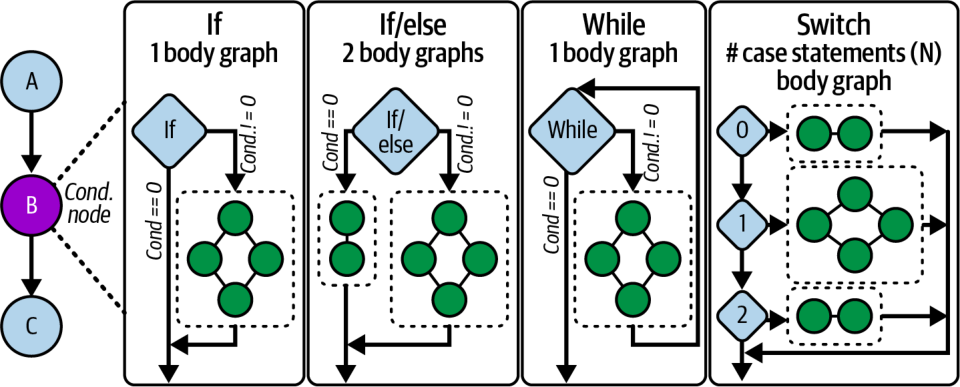
\includegraphics[width=\linewidth]{figs/fig12-9.png}\\
    {\scriptsize Figure 12-9. Conditional node types: IF, IF/ELSE, WHILE, SWITCH}
  \end{columns}
  \smallskip
  \pe{the recorded show gains ``choose your own adventure'' buttons --- and the GPU presses them.}
\end{frame}

% ---------------------------------------------------------------- 17
\begin{frame}{Dynamic Parallelism: Kernels That Launch Kernels}
  \begin{columns}[c]
    \column{0.55\textwidth}
    \begin{itemize}
      \item Graphs replay \kw{known} pipelines. When the \emph{shape of the work emerges from
            the data} --- graph traversal, adaptive mesh, hierarchical reduction ---
            you can't prerecord it.
      \item \kw{DP}: a parent kernel inspects its own output and launches \kw{child kernels}
            on the device (compile with \texttt{-rdc=true}).
      \item LLM example: most tokens take the standard path; a DP kernel tail-launches an
            auxiliary attention block \kw{only for the tokens that need it}.
      \item Telltale profile: \texttt{Kernel A $\to$ GPU idle gap $\to$ Kernel B},
            where the gap is the CPU deciding.
    \end{itemize}
    \column{0.42\textwidth}
    \centering
    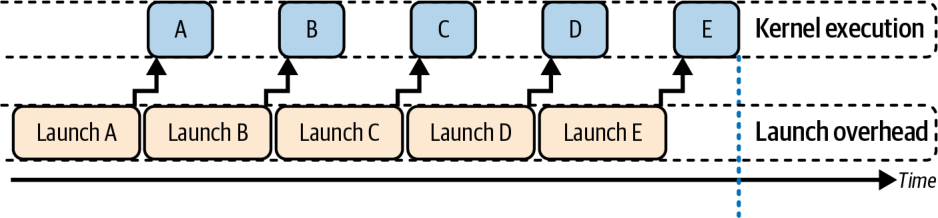
\includegraphics[width=\linewidth]{figs/fig12-12.png}\\[2pt]
    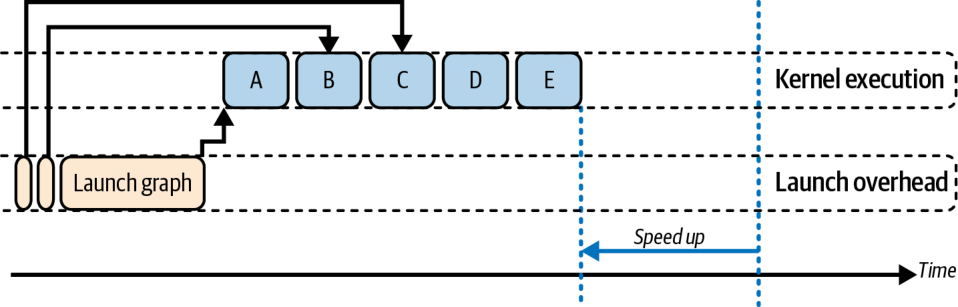
\includegraphics[width=\linewidth]{figs/fig12-13.png}\\
    {\scriptsize Figures 12-12 / 12-13. Host-driven gaps (top) vs.\ device-side launches (bottom)}
  \end{columns}
\end{frame}

% ---------------------------------------------------------------- 18
\begin{frame}[fragile]{Dynamic Parallelism: Numbers and Caveats}
  \begin{columns}[t]
    \column{0.5\textwidth}
    {\small
    \begin{tabular}{@{}lrr@{}}
      \toprule
      \textbf{Metric (2 children)} & \textbf{Host} & \textbf{Device} \\
      \midrule
      Host launches & 3 & \kw{1} \\
      Overhead per launch & $\sim$20 \textmu s & $\sim$25 \textmu s \\
      GPU idle during sequence & $\sim$40\% & \kw{$\sim$5\%} \\
      Total runtime & 1.00 ms & \kw{0.75 ms} \\
      \bottomrule
    \end{tabular}}\\[4pt]
    {\scriptsize Table 12-2 (illustrative\refmark{7}). Bonus: intermediates \kw{stay in GPU memory} --- better locality.}
    \column{0.47\textwidth}
    \begin{itemize}\small
      \item Parent implicitly \kw{waits for all children} --- no device-side
            \texttt{cudaDeviceSynchronize()} needed (host syncs the stream once).
      \item Child launches consume \kw{stack space} and pending-launch slots;
            default cap \kw{2{,}048 pending} children --- both raised via
            \texttt{cudaDeviceSetLimit}.
      \item Device launch $\approx$ host launch in overhead: \kw{tiny children lose}.
            Fixed, repeated flow? Prefer \kw{device-launched graphs} --- they amortize.
    \end{itemize}
  \end{columns}
  \medskip
  \pe{DP is for work you can't predict; graphs are for work you can.}
\end{frame}

% ---------------------------------------------------------------- 19
\begin{frame}{Scaling Out: Overlap Communication with Compute}
  \begin{itemize}
    \item Multi-GPU goal is unchanged: \kw{hide data movement behind useful work}.
          NVLink is fast; it is still not HBM --- overlap or plateau.
    \item \kw{Peer-to-peer}: \texttt{cudaMemcpyPeerAsync(dst, dstGpu, src, srcGpu, size, commStream)}
          on a second stream while compute streams keep running.
    \item \kw{NCCL}: nonblocking collectives (all-reduce rings/trees) saturate NVLink/NVSwitch
          alongside compute streams --- the engine of PyTorch DDP.
    \item \kw{CUDA-aware MPI}: pass device pointers to \texttt{MPI\_Send};
          \kw{GPUDirect RDMA} moves data NIC$\to$HBM over InfiniBand, no host staging.
    \item Context: a GB200 \kw{NVL72} rack = 72 GPUs in one NVLink domain, up to
          \kw{30 TB} unified memory --- one giant coprocessor if software keeps up.\refmark{1}
  \end{itemize}
  \medskip
  \pe{without overlap, scaling stops the moment communication time equals compute time; with overlap, 4 GPUs can look like one 4$\times$-faster GPU.}
\end{frame}

% ---------------------------------------------------------------- 20
\begin{frame}[fragile]{NVSHMEM: GPUs Read and Write Each Other's Memory}
  \begin{columns}[c]
    \column{0.52\textwidth}
    \begin{itemize}
      \item \kw{PGAS} model: each GPU is a \kw{PE} (processing element) in a partitioned
            global address space; device code does \kw{one-sided put/get} into a peer's memory.
      \item Classic \kw{send-and-signal}:
    \end{itemize}
\begin{lstlisting}
// GPU 0 kernel:
nvshmem_float_p(remote_data + 1, value, dest_pe); // put
nvshmem_quiet();                     // ensure completion
nvshmem_int_p(remote_flag, 1, dest_pe);   // raise flag
// GPU 1 kernel:
nvshmem_int_wait_until(remote_flag, NVSHMEM_CMP_EQ, 1);
float val = remote_data[1];          // payload is valid
\end{lstlisting}
    \column{0.44\textwidth}
    \centering
    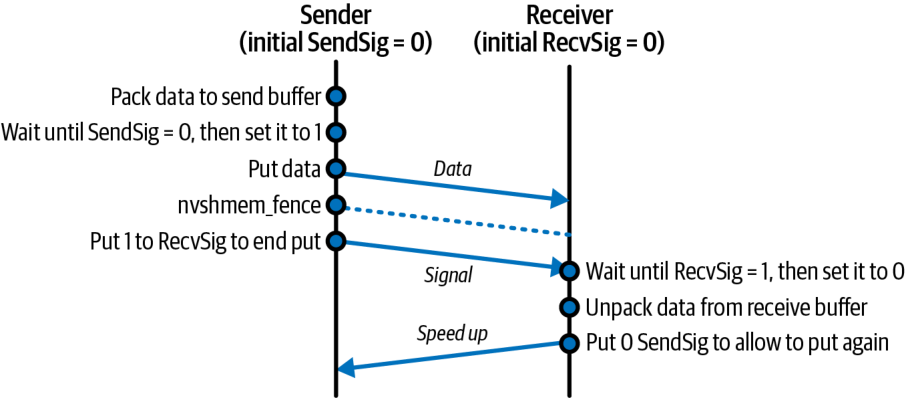
\includegraphics[width=\linewidth]{figs/fig12-14.png}\\
    {\scriptsize Figure 12-14. NVSHMEM one-sided communication}
    \medskip
    \begin{itemize}\small
      \item No CPU, no kernel-launch overhead: a multistep exchange becomes
            \kw{one hardware transaction} at near wire speed.
    \end{itemize}
  \end{columns}
  \medskip
  \pe{instead of mailing packages through the post office (CPU), GPUs walk over and put things directly on each other's desks.}
\end{frame}

% ---------------------------------------------------------------- 21
\begin{frame}[fragile]{NVSHMEM Patterns: Pipelines, Work Stealing, Lockstep}
  \begin{columns}[t]
    \column{0.5\textwidth}
    \begin{itemize}\small
      \item \kw{Two-stage pipeline}: GPU 0 computes attention, \kw{puts} activations to GPU 1
            + signals; GPU 1's persistent kernel starts the MLP while GPU 0 moves to the
            next batch --- handoffs \kw{hidden behind compute}.
      \item \kw{Device-side work stealing}:
    \end{itemize}
\begin{lstlisting}
while (true) {
  int idx = nvshmem_int_atomic_inc(queue_head);
  if (idx >= N_tasks) break;
  // process tasks[idx] ...
}
\end{lstlisting}
    \column{0.46\textwidth}
    \begin{itemize}\small
      \item \kw{Lockstep steps}: launch one cooperative kernel on all PEs with
            \kw{\texttt{nvshmemx\_collective\_launch()}} (required for device-side
            barriers/collectives), then \texttt{nvshmem\_barrier\_all()} inside.
      \item \kw{Don't over-synchronize}: global barriers stall everyone on the slowest peer ---
            prefer point-to-point signals (\texttt{nvshmem\_signal\_*}).
      \item Shines for \kw{irregular} work: graph algorithms, dynamic load balancing,
            event-driven simulation.
      \item NVSHMEM kernels \kw{can be captured} inside CUDA Graphs.
    \end{itemize}
  \end{columns}
\end{frame}

% ---------------------------------------------------------------- 22
\begin{frame}[fragile]{NCCL Inside CUDA Graphs: Deterministic Training Steps}
  \begin{columns}[c]
    \column{0.52\textwidth}
\begin{lstlisting}
cudaStreamBeginCapture(captureStream,
    cudaStreamCaptureModeGlobal);
forwardKernel<<<..., captureStream>>>(...);
ncclAllReduce(sendBuf, recvBuf, count, ncclFloat,
    ncclSum, comm, captureStream);
backwardKernel<<<..., captureStream>>>(...);
cudaStreamEndCapture(captureStream, &graph);
// instantiate + upload once; then per step:
cudaGraphLaunch(graphExec, captureStream);
\end{lstlisting}
    \begin{itemize}\small
      \item \kw{Bucketed all-reduce}: split gradients across streams inside the capture ---
            comm on stream B overlaps compute on stream A (Figure 12-15).
    \end{itemize}
    \column{0.44\textwidth}
    \begin{itemize}\small
      \item NCCL calls become \kw{graph nodes}; per-step host work drops to
            \kw{one \texttt{cudaGraphLaunch}} --- less CPU load, less \kw{launch jitter}.
      \item Rules: \kw{all ranks} capture and replay the \kw{same sequence, same communicator}
            --- mismatch risks \kw{deadlock} or silent corruption.
      \item Run \kw{warm-up collectives} before capture to initialize communicators.
      \item At cluster scale these savings \kw{compound}: tighter sync, higher utilization.
    \end{itemize}
  \end{columns}
  \medskip
  \pe{everyone in the orchestra plays from the same recorded score --- if one violinist improvises, the concert deadlocks.}
\end{frame}

% ---------------------------------------------------------------- 23
\begin{frame}{Roofline-Guided Orchestration: Which Tool, When}
  \begin{columns}[c]
    \column{0.55\textwidth}
    \begin{itemize}\small
      \item \kw{Memory-bound} (left of ridge): overlap is king --- async copies, streams,
            concurrent kernels; \kw{reduce bytes} with FP16/FP8/FP4. (Fusion helps only modestly.)
      \item \kw{Compute-bound but under the roof}: kill launch overhead ---
            \kw{fusion, persistent kernels, CUDA Graphs, device-side launches} push you toward the flat ceiling.
      \item \kw{Neither} (mid-chart): \kw{increase concurrency} --- multiple kernels/streams/graphs
            in parallel raise the aggregate point on both axes.
    \end{itemize}
    \column{0.42\textwidth}
    \centering
    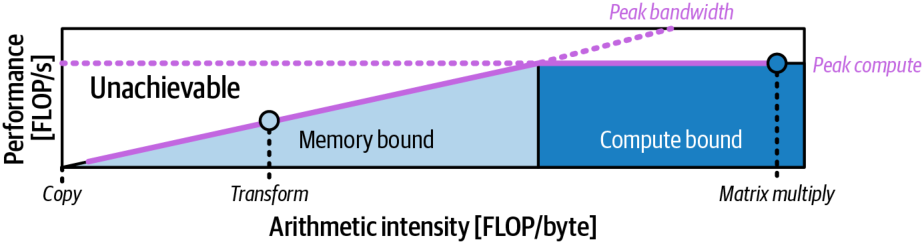
\includegraphics[width=\linewidth]{figs/fig12-17.png}\\
    {\scriptsize Figure 12-17. Two ceilings: memory roof (sloped), compute roof (flat)}
  \end{columns}
  \medskip
  \begin{block}{The takeaway}
    Count FLOPs and bytes with Nsight Compute, plot the point, \kw{then} pick the technique ---
    and re-measure after every change. Roofline guides; \kw{profiling verifies}.
  \end{block}
\end{frame}

% ---------------------------------------------------------------- 24
\begin{frame}{Key Takeaways}
  \begin{columns}[t]
    \column{0.48\textwidth}
    \begin{itemize}\small
      \item \kw{Atomic work queues}: L2 atomics + batched increments balance irregular work
            on-device --- up to 2$\times$ in extreme imbalance, 10--30\% typical.
      \item \kw{CUDA Graphs}: capture once, replay with one call --- typically
            \kw{20--30\% latency reduction} for launch-bound pipelines; static addresses required.
      \item \kw{Device-side orchestration}: device-launched graphs (tail / fire-and-forget /
            sibling), conditional nodes, and DP keep decision + dispatch on the GPU.
    \end{itemize}
    \column{0.48\textwidth}
    \begin{itemize}\small
      \item \kw{DP vs.\ graphs}: DP for work that \emph{emerges from data};
            graphs for \emph{repeated, known} flow.
      \item \kw{Multi-GPU}: always overlap --- peer copies, NCCL in graphs, CUDA-aware MPI,
            NVSHMEM one-sided ops; near-linear scaling needs the CPU off the critical path.
      \item \kw{Roofline first}: memory-bound $\to$ overlap + fewer bytes;
            compute-bound $\to$ fewer launches; in-between $\to$ more concurrency.
    \end{itemize}
  \end{columns}
\end{frame}

% ---------------------------------------------------------------- 25
\begin{frame}{Conclusion and What's Next}
  \begin{block}{This chapter in one sentence}
    Fast kernels aren't enough --- \kw{orchestration} (queues, graphs, device-initiated launches,
    GPU-to-GPU memory sharing) is what keeps every SM fed and the CPU out of the loop.
  \end{block}
  \begin{itemize}
    \item Hardware is dissolving the CPU--GPU boundary (Grace Blackwell, Vera Rubin, coherent
          NVLink) --- but \kw{software} still has to exploit it; these techniques are how.
    \item Next chapter (13): how \kw{PyTorch} packages these ideas --- streams, graphs, async ops,
          optimized kernels --- into a few lines of Python.
    \item Pairs with my Chapter 6 talk: first \kw{fill} the GPU (occupancy),
          then \kw{never let it drain} (orchestration).
  \end{itemize}
  \medskip
  \centering\itshape Questions?
\end{frame}

% ---------------------------------------------------------------- 26
\begin{frame}{References \& Further Reading}
  {\footnotesize
  \begin{enumerate}
    \item C.\ Fregly. \emph{AI Systems Performance Engineering} (O'Reilly, 2026), Chapter 12;
          NVIDIA GB200 NVL72 product page (72-GPU NVLink domain, 30 TB unified memory).
    \item NVIDIA. \emph{CUDA C++ Programming Guide} --- CUDA Graphs, stream capture,
          \texttt{cudaGraphExecUpdate}, dynamic parallelism, device runtime limits.
    \item NVIDIA Developer Blog. \emph{Enabling Dynamic Control Flow in CUDA Graphs with
          Device Graph Launch} --- device-initiated launches, fire-and-forget / tail / sibling modes.
    \item NVIDIA Developer Blog. \emph{Dynamic Control Flow in CUDA Graphs with Conditional Nodes}
          (CUDA 12.4+) --- IF / IF-ELSE / WHILE / SWITCH nodes.
    \item NVIDIA. \emph{NVSHMEM documentation} --- PGAS model, one-sided put/get, signals,
          \texttt{nvshmemx\_collective\_launch}; \emph{NCCL documentation} --- graph-captured collectives.
    \item PyTorch Blog. \emph{Accelerating PyTorch with CUDA Graphs} ---
          \texttt{torch.cuda.CUDAGraph}, static memory pools, \texttt{reduce-overhead} compile mode.
    \item Book code and benchmarks: the book's GitHub repository (per-architecture results for the
          illustrative tables in this deck).
  \end{enumerate}}
\end{frame}

\end{document}
